\chapter{Conclusions and recommendations for future work}

\ifpdf
    \graphicspath{{Chapter7/figs/raster/}{Chapter7/figs/pdf/}{Chapter7/figs/}}
\else
    \graphicspath{{Chapter7/figs/vector/}{Chapter7/figs/}}
\fi
\section{Introduction}

This PhD has made advances in several aspects of multi-scale modelling of 
granular flows and understanding the complex rheology of dry and submerged 
granular flows. The significant contributions of this PhD are summarised in 
this chapter.

\subsection{Multi-scale modelling of dry granular flows}

The granular flow problem is modelled using material point method, a continuum 
approach, and at the grain-scale level using discrete element technique. In the 
present study, a two-dimensional DEM code is developed in C++ to study the 
micro-scale rheology of dry granular flows. A Verlet-list algorithm is adopted 
for neighbourhood detection to improve the computational efficiency. A 
linear-elastic contact model with a frictional contact is used to model rapid 
granular flows. A sweep-line Voronoi tesselation algorithm is implemented in 
the present study to extract continuum properties such as packing density from 
the local grain-scale simulations.

In order to capture the macro-scale response, a template-based 
three-dimensional C++ Material Point Method code, an Eulerian-Lagrangian 
approach, developed at the University of Cambridge is modified and extended to 
study granular flows as a continuum. In the present study, the Generalised 
Interpolation Material Point GIMP method is implemented to reduce the 
cell-crossing noise and oscillations observed during large-deformation problem, 
when using the standard MPM. The three-dimensional MPM code is parallelised to 
run on multi-core systems, thus improving the computational efficiency. The 
algorithm of the MPM code is improved to handle multi-body dynamics and 
interactions. In the present study, constitutive models, such as NorSand and 
Bingham fluid were implemented in MPM. Various smoothing/averaging techniques, 
such as BBar approach were implemented. This dissertation includes only those 
results from two-dimensional plane-strain granular flow problems. The 
multi-scale tools developed in the present study is used to understand the 
capability and limitations of continuum approach in modelling dry granular 
flows.

\subsubsection*{Granular column collapse}

Multi-scale simulation of dry granular flows are performed to capture the 
local rheology, and to understand the capability and limitations of continuum 
models in realistic simulation of granular flow dynamics. For short columns, 
the run-out distance is found to be proportional to the granular mass above the 
failure surface. The spreading results from a Coulomb-like failure of the 
edges. The continuum approach, using a simple frictional dissipation model, is 
able to capture the flow dynamics of short columns. However, the collapse of 
tall columns is characterised by an initial collisional regime and a power-law 
dependence between the run-out and the initial aspect ratio of the granular 
column is observed. The energy evolution study reveals that the lack of 
collisional dissipation mechanism in the MPM simulations results in a 
substantially longer run-out distance for large aspect ratio columns. This 
shows that continuum approach using frictional laws are able to capture the 
flow kinematics at small aspect ratios, which is characterised by an inertial 
number \textit{I} less than 0.2 indicating a dense granular flow. However, 
continuum approach like MPM are unable to precisely describe the flow dynamics 
of tall columns, which is characterised by an initial collisional regime 
(\textit{I} > 0.2). DEM studies on the role of initial material properties 
reveal that the initial packing fraction and the distribution of kinetic energy 
in the system have a significant influence on the flow kinematics and the 
run-out behaviour. For the same material, a dense granular packing results in a 
longer run-out distance in comparison to the initially loose granular column. 
Hence it is important to consider macroscopic parameters like packing fraction, 
which are due to meso-scale grain arrangements, when modelling the granular 
system as a continuum.

\subsubsection*{Granular slopes subjected to impact loading}

The ability of MPM in modelling transient flows that does not involve collision 
is further investigated. The distribution of kinetic energy in the granular 
mass is found to have a significant effect on the flow kinematics. In the 
present study, a multi-scale analyses of a granular slope subjected to 
impact velocities reveals a power-law dependence of the run-out distance and 
time as a function of the input energy with non-trivial exponents. The 
power-law behaviour is found to be a generic feature of granular dynamics. Two 
different regimes are observed depending on the input energy. The low energy 
regime reflects mainly the destabilisation of the pile, with a run-out time 
independent of the input energy. The high energy regime involves spreading 
dynamics, which is characterised by a decay time that is defined as the time 
required for the input energy to  decline by a factor $1/2$. MPM is 
successfully able to simulate the transient evolution with a single 
input parameter, the macroscopic friction angle. This study exemplifies the 
suitability of MPM, as a continuum approach, in modelling large-deformation 
granular flow dynamics and opens the possibility of realistic simulation of 
geological-scale flows on complex topographies.


The distribution of the kinetic energy in the system is found to have a 
significant influence in the low energy regime, where a large 
fraction of the input energy is consumed in the destabilisation process. 
However at higher input energy, where most of the energy is dissipated during 
the spreading phase, the run-out distance has a weak dependence on 
the distribution of velocity in the granular mass. The material characteristics 
of the granular slope affect the constant of proportionality and not the 
exponent in the power-law relation between the run-out and the input energy. 

\subsection{Granular flows in fluid}

A two-dimensional coupled lattice Boltzmann - DEM technique is developed in C++ 
to understand the local rheology of granular flows in fluid. A multi-relaxation 
time LBM approach is implemented in the present study to ensure numerical 
stability. The coupled LBM--DEM technique offers the possibility to capture the 
intricate micro-scale effects such as the hydrodynamic instabilities. Coupled 
LBM-DEM involves modelling interactions of a few thousand soil grains with a 
few million fluid nodes. Hence, in the present study the LBM-DEM approach is 
implemented in the General Purpose Graphical Processing Units. The GPGPU 
implementation of the coupled LBM -- DEM technique offers the capability to 
model large scale fluid -- grain systems, which are otherwise impossible to 
simulate using conventional computational techniques. In the present study, 
simulations involving up to 5000 soil grains interacting with 9 million LBM 
fluid nodes are modelled. Efficient data transfer mechanisms that achieves 
coalesced global memory ensures that the GPGPU implementation scales linearly 
with the domain size. Granular flows in fluid involves soil grains interacting 
with fluid resulting in formation of turbulent vortices. In order to model the 
turbulent nature of granular flows, the LBM-MRT technique is coupled with the 
Smagorinsky turbulent model. 

\section{Recommendations for future research}
This research work involves the following stages: (1) understanding the limits 
of the continuum and the discrete-element approaches in modelling the granular 
flow, and investigating the influence of various microscopic parameters on the 
macroscopic flow behaviour, (2) understanding the 
differences in the mechanism of the granular flows in dry and submerged 
conditions, and (3) Modelling the granular flow behaviour using the $\mu(I)$ 
rheology for dry and submerged flow conditions.

\subsection{Multi-scale simulations of granular flows}
The continuum and discrete-element simulations of the dry and the submerged 
granular flows will be performed to understand the differences in their flow 
mechanism. Multi-scale analyses of granular flows enable us to understand the 
limitations of the continuum approach in modelling large deformation granular 
flow problems, and help us to identify the micro-scale parameters responsible 
for the complex macroscopic behaviour. Multi-scale modelling of the collapse of 
a granular columns on a horizontal surface have been performed. Continuum 
simulations accurately predict the granular flow behaviour for columns with 
smaller aspect ratios, however they fail to capture the dynamics of the flow 
for columns with larger aspect ratios. 

In order to understand the difference in the flow dynamics with increasing 
aspect ratios, further analyses will be performed to study the mechanism of 
energy dissipation in the particle scale, i.e. the evolution of kinetic energy 
and potential energy with time. A simple mathematical relationship based on the 
initial potential energy of the grains lying above the failure surface is being 
developed to describe the flow dynamics of the granular column collapse problem 
with different aspect ratios. The relationship will enable us to understand the 
variation in the flow dynamics in the continuum and the particle-scale. The 
continuum description of granular column collapse showed non-physical behaviour 
near the foot of the column, further analyses will be carried out to understand 
the effect of interface properties on the run-out distance. Further details on 
the continuum modelling of granular flow are presented in the next section. 
Micro-scale parameters influencing the flow dynamics will be identified and the 
influence of these parameters on the deposit morphology will be investigated. 
Multi-scale analysis of large deformation flow problem such as flow of dry 
granular materials down an inclined flume will be performed. This analysis will 
provide an insight on the limits of the continuum approach in modelling large 
deformation problems, which involve large shear-rates. The results from the 
analysis will be compared with the experimental results 
of~\citet{Denlinger2001} on miniature flume experiments. The influence of 
parameters, such as particle size, density, packing and dilatancy, on the flow 
dynamics will be explored. These studies will be useful in describing the 
granular flow behaviour using the $\mu(I)$ rheology.

In order to understand the differences in the mechanism between the dry and the 
submerged granular flows, multi-scale analysis of granular flows in fluid will 
be performed. In particle-scale approach, the Discrete Element Method technique 
coupled with Lattice Boltzmann approach will be adopted to study the collapse 
of granular columns in fluids. Dynamic fluid-coupling in the Material Point 
Method will be developed to study the behaviour of granular flows in fluids. 
The numerical simulations will be verified with the experimental results 
of~\cite{Cassar2005} on immersed granular flows. The effect of packing density 
of granular material, frictional parameters and the viscosity of the fluid on 
the flow dynamics and the phase-transition behaviour will also be investigated. 
The influence of the fluid viscosity on the flow behaviour will also be 
investigated. The variation in the flow dynamic and the deposit morphology for 
dry and submerged granular flows will also be analysed. The parameters that 
cause a change in the flow dynamic between the dry and the submerged flow 
conditions will be used in extending the $\mu(I)$ rheology for submerged 
granular flows. 


\subsection{Developments in Material Point Method}
The present MPM code is capable of solving the granular flow problems using the 
Mohr-Coulomb constitutive model. It is also capable of solving seepage problems 
with static fluid-solid interface. In the present study, the Material Point 
Method will be extended to solve 3D problems and it will be implemented into a 
standard framework, similar to the Finite Element framework developed in the 
University of Cambridge. Constitutive models such as Nor-Sand and $\mu(I)$ 
rheology will be implemented to model the dense granular flows. Modified 
Nor-Sand constitutive model~\citep{Robert2010} implemented in the present study 
will be validated by performing element testing and the results will be 
verified with the results of~\citet{Jefferies2005a}. The current MPM code is 
capable of simulating only small deformation problems, however special 
attention is required in modelling large deformation problems, especially those 
involving two-phase systems. Objective stress rate such as Jaumann stress rate 
has been implemented to study large deformation problems. The dynamic 
re-meshing technique~\citep{Shin2010a} will be implemented to efficiently solve 
large deformation problems. The dynamic meshing approach is useful for problems 
involving motion of a finite size body in unbounded domains, in which the 
extent of material run-out and the deformation is unknown a priori. The 
approach involves searching for cells that only contain material points, 
thereby avoiding unnecessary storage and computation. 

The present fluid coupling algorithm in the MPM involves only static 
boundaries, and conserves the equation of momentum for fluid particles by 
introducing additional particles in a cell, when the number of particles 
decreases. A dynamic solid-fluid interface modelling in the Material Point 
Method will be developed. The approach involves the following steps: 
identification of the soil particles along the boundary of the current soil 
domain, obtaining the nodal numbers for the edges of each soil particle and 
definition of a new boundary (see Figure~\ref{fig:MPMFluidB}). The shape of the 
boundary is approximated by equivalent rectangular grids, similar to the 
coupling technique adopted in the discrete-element approach. The procedure is 
repeated until the entire boundary is defined. This process is repeated for 
each time step to simulate the dynamic boundary behaviour which is common in 
the case of granular flows in a fluid. 

The MPM code will be extended to include the phase-transition behaviour in a 
continuum domain for partially fluidized granular flows~\citep{Aranson2002, 
Aranson2001, Volfson2003}. The theory is based on the hydrodynamics of the 
flow, coupled with an order parameter equation, which describes the transition 
between the flowing and the static components of the granular system. The order 
parameter is defined as a fraction of static contacts among all contacts 
between particles. The shear stresses in a partially fluidized granular matter 
is assumed to have two components: the dynamic part that is proportional to the 
shear strain rate and the strain-independent or the static part. The ratio of 
these two parts is a function of the order parameter. The relative magnitude of 
the static shear stress is controlled by the order parameter which varies from 
0 in the liquid phase to 1 in the solid phase.

\begin{figure}[htbp]
\centering
\includegraphics[width=0.95\textwidth]{MPMFluidB}
\caption{Identification of dynamic solid-fluid 
boundary}
\label{fig:MPMFluidB}
\end{figure}

\subsection{The I rheology}

The $\mu(I)$ rheology is capable of describing the behaviour of dense granular 
flows. However, it considers the yield strength as an adjustable rheological 
property, which contradicts the basic understanding that the
strength evolves as the debris-flow motion progresses. Also, the $\mu(I)$ 
rheology uses the Mohr-Coulomb constitutive model to describe the yielding of 
granular materials. In the present study, the evolution of soil strength 
with time will be considered using models based on critical state framework. 
Nor-Sand constitutive model will be implemented in the present study to 
describe the plastic flow of granular materials. The $\mu(I)$ rheology will be 
extended to describe the behaviour of granular flows in fluids. In the case of 
dense granular flows, the parameter \textit{I} is described as the ratio 
between the time taken for a particle to fall into the hole, $t_{micro}$, and 
the meantime, $t_{mean}$, which is inversely related to the shear rate. If the 
velocity of the ambient fluid is low, then the time taken by the particle to 
fall into a hole, is then controlled by the viscosity of the ambient 
fluid~\citep{Pouliquen2005}. The $\mu(I)$ rheology will be modified to include 
the effect of fluid viscosity to model granular flows in fluids based on the 
parameters identified to control the flow dynamics.

\subsection{Homogenization of granular flows}
Granular materials are composed of grains in contact, and are therefore 
discontinuous and heterogeneous. The macroscopic material properties of these 
materials are liked to the fabric of the medium. It is interesting to define 
the behaviour of granular materials at the macroscopic scale from 
characteristics defined at the local scale. This approach has been widely 
developed for heterogeneous continuum and is known as the homogenization 
method. This kind of approach is different from the phenomenological one, in 
which the constitutive model is derived from the general laws of 
thermodynamics. These phenomenological models introduce some material 
parameters whose values are obtained from the simulations performed on 
representative volume element. The main objective of the homogenization method 
is to obtain a constitutive relation at the scale of a representative volume 
element, based the information on the material behaviour at the micro-scale and 
the micro-structure. For granular media, the micro-scale is generally the grain 
scale. The scale of the representative volume element is of several orders of 
magnitude higher. The homogenization process is based on three relations, a 
localization operator, a local constitutive law and an averaging operator, see 
Chapter 6. An intrinsic difficulty in the case of granular materials arise from 
the fact that the variables at the micro-scale and the macro-scale are of 
different nature. At the micro-scale the material behaviour is described using 
vectorial variables such as contact forces, grain displacement and grain 
rotation, where as the macroscopic behaviour law uses tensorial variables 
(stress tensor, strain tensor). The micro-polar plasticity constitutive 
formulation~\citep{Suiker2001} that is directly related to micro-scale 
properties, such as contact stiffness, particle density, particle radius and 
its micro-structure will be extended to large scale deformation problems which 
involves loss or gain of contacts between grains. Discrete Element Method 
simulations provide useful insight on the role of contact forces at 
micro-scale. The macroscopic stress is related to microscopic contact forces 
using the virtual work theorem. The microscopic kinematic variables usually 
considered are the displacement of the centre of mass of the particle and the 
ration of the particle. The local phenomena occurring at the micro-scale during 
the deformation of granular material are complex. Different approaches have 
been proposed in the literature to establish the link between particle-level 
displacements and macro-scale deformations. The micro-behaviour is converted 
into a macroscopic model through the conservation of internal work. The local 
constitutive law gives the value of contact forces and the average over the 
sample provides the value of the stress tensor. 

\subsection{Slopes subjected to impact}
This work may be pursued along two directions: 1) experimental realization of a 
similar setup with different modes of energy injection and 2) investigating the 
effect of various particle shapes or the presence of an ambient fluid. Although 
numerical simulations are generally reliable with realistic results found in 
the past studies of steady flows, we believe that the transients are more 
sensitive situations than steady states and the  experiments are necessary for 
checking the validation of the results suggested by the simulations. Provided a 
convenient method is used for supplying kinetic energy homogeneously into a 
pile, our configuration is also interesting for the investigation of the 
behavior of a pile immersed in a viscous fluid.